\documentclass[letterpaper,11pt]{article}
\usepackage[spanish]{babel}
\usepackage[utf8]{inputenc}
\usepackage{graphicx}
\usepackage{amsfonts,amsmath,amssymb,float, amsthm,mathrsfs}  
\usepackage[right=4.5cm,left=2cm,top=3cm,bottom=3cm,headsep= 0.7cm,footskip=0.5cm]{geometry}
\usepackage{enumerate}
\usepackage{wrapfig} 
\usepackage[rflt]{floatflt} 
\usepackage{framed}
%\usepackage[most]{tcolorbox}
\usepackage[dvipsnames]{xcolor}
\colorlet{shadecolor}{green!20}
\setlength\FrameSep{0.5ex}
\usepackage{thmtools}
\usepackage{esint}
\usepackage{cancel}
\usepackage{listings} 
\usepackage{pstricks, caption}
\usepackage[colorlinks]{hyperref}
\usepackage{csquotes}
\usepackage{fullpage}
\usepackage{enumitem}
\usepackage{etoolbox}
\usepackage{tikz}
\usepackage{tikz-3dplot}
\tdplotsetmaincoords{80}{70}
\usetikzlibrary{decorations.markings}
\usetikzlibrary{arrows,babel}
\usepackage[font=small]{caption}
\usepackage{scalerel} %\scaleto{text}{size}
\usepackage{fancyhdr}
\usepackage{comment}
\usepackage{marginnote}
\usepackage{tensor}
\usepackage{cleveref}
\newcommand{\dbar}{\mathchar'26\mkern-12mu d}
\renewcommand*{\marginnotevadjust}{-0.1cm}
\renewcommand*{\marginfont}{\footnotesize}
\setlength{\headheight}{15pt}
\addtolength{\topmargin}{-14.49998pt}
\setlength{\headsep}{15pt}
\setlength{\footskip}{14.49998pt}
\decimalpoint
\newcommand{\grad}{^\circ}
\newlength{\drop}
\DeclareMathOperator{\sign}{sgn}
\DeclareMathOperator{\Log}{Log}
\providecommand{\norm}[1]{\lVert#1\rVert}
\usepackage{subcaption}

\let\cancelorigcolor\CancelColor% Just for conveniency...

\newcommand{\CancelTo}[3][]{%
  \ifblank{#1}{}{%
    \renewcommand{\CancelColor}{#1}%
  }
  \cancelto{#2}{#3}% 
}


\begin{document}

\pagestyle{plain}

\begin{flushleft}\vspace{-2cm}
Departamento de Física \\
Facultad de Cs. Físicas y Matemáticas\\
Universidad de Concepción
\end{flushleft}

\begin{flushright}\vspace{-1.5cm}
\textbf{Tópicos en Relatividad General} 
\end{flushright}



\rule{\linewidth}{0.1mm}

\begin{center}
\textbf{\LARGE Semana 7}
\end{center}

\begin{flushleft}
\textbf{Nombre:} Alejandro Saavedra San Martín. \\
\textbf{Profesor:} Guillermo Rubilar Alegría.
\end{flushleft}

\section*{Ejercicio 1:}

Considere un espaciotiempo estático esféricamente simétrico, de modo que, en coordenadas de curvatura, el elemento de línea se expresa en la forma
\begin{equation}
ds^2 = A(r) (c \, dt)^2 - B(r) dr^2 - r^2(d\theta^2 + \sin^2\theta d\varphi^2), \quad A > 0, B > 0. \label{eq:ej-1-metric}
\end{equation}


\textbf{(a)} Considere un observador ``en reposo", en el sentido que sus coordenadas espaciales $(r,\theta,\varphi)$ son siempre constantes. Además, debido a la simetría esférica, pueden elegirse sus coordenadas angulares como $\theta_{\text{obs}} = \pi/2$ y $\varphi_{\text{obs}} = 0$. Determine la expresión para la línea de mundo de este observador, parametrizada usando su tiempo propio, es decir, determine $x_{\text{obs}}^{\mu}(\tau_{\text{obs}})$, en términos de $A$, $B$ y $r$.
\\

\textbf{Solución:} Un dibujo esquemático de la situación física se encuentra en la figura \ref{fig:Ej-1.1}. Las coordenadas del observador son $x_{\text{obs}}^{\mu}(\tau_{\text{obs}}) = (c t_{\text{obs}}(\tau_{\text{obs}}),r,\pi/2,0)$, con $r = \text{cte}$. Para encontrar $t_{\text{obs}}(\tau_{\text{obs}})$ debemos recordar la siguiente relación entre el tiempo propio y el elemento de línea:
\begin{equation}
c^2 d\tau^2 = ds^2 = g_{\mu\nu} dx^{\mu} dx^{\nu}.
\end{equation}

Evaluando los coeficientes de la métrica \eqref{eq:ej-1-metric} y considerando que la única coordenada no constante es $t$, tenemos que
\begin{equation}
c^2d\tau^2 = g_{tt} c^2dt^2 = A(r) c^2 dt^2.
\end{equation} 

Despejando $dt/d\tau$, obtenemos
\begin{equation}
\frac{dt}{d\tau} = \frac{1}{\sqrt{A(r)}} .
\end{equation}

Integrando con respecto a $\tau$:
\begin{equation}
t = \frac{\tau}{\sqrt{A(r)}} + C,
\end{equation}
donde $C$ es una constante de integración. Si asumimos que el observador se encuentra en el evento $x^{\mu} = (0,r,\pi/2,0)$ para $\tau = 0$, se fija la constante $C$ a cero. Entonces, renombrando las variables $t \to t_{\text{obs}}$ y $\tau \to \tau_{\text{obs}}$, 
\begin{equation}
t_{\text{obs}}(\tau_\text{obs}) = \frac{\tau_\text{obs}}{\sqrt{A(r)}}.
\end{equation}

Por lo tanto, la línea de mundo se encuentra parametrizada por
\begin{shaded}
\begin{equation}
x_{\text{obs}}^{\mu}(\tau_\text{obs}) = \left(\frac{c\tau_\text{obs}}{\sqrt{A(r)}},r,\frac{\pi}{2},0 \right). \label{eq:ej-1-a)}
\end{equation}
\end{shaded}

\textbf{(b)} Considere ahora fotones (rayos de luz) confinados (usando, por ejemplo, fibra óptica) a moverse en una circunferencia (es decir, con coordenada radial constante), también con $\theta_{\text{fot}} = \pi/2$. Determine la expresión para la línea de mundo de estos fotones, parametrizada en términos del ángulo $\varphi_{\text{fot}}$ a lo largo de su trayectoria. Asuma que para $\varphi_{\text{fot}} = 0$ el fotón pasa por el evento con coordenadas $x^{\mu}(0) = (0,r,\pi/2,0)$ (que también está en la línea de mundo del observador).
\\

\textbf{Solución:} Las coordenadas del fotón son $x_{\text{fot}}^{\mu}(\lambda) = (ct_{\text{fot}}(\lambda),r,\pi/2,\varphi_{\text{fot}}(\lambda))$. Elegimos parametrizar su línea de mundo por $\lambda = \varphi_{\text{fot}}$. 

Usando la condición de curvas nulas para el fotón:
\begin{equation}
ds^2|_{\text{fot}} = g_{\mu\nu} dx^{\mu}dx^{\nu} = 0.
\end{equation}

Evaluamos los coeficientes de la métrica \eqref{eq:ej-1-metric}  considerando que las únicas coordenadas no constantes son $ct$ y $\varphi$,
\begin{align}
g_{\mu\nu} dx^{\mu}dx^{\nu} &= 0 \\
g_{tt} c^2dt^2 + g_{rr} \CancelTo[\color{red}]{0}{dr^2} + g_{\theta\theta} \CancelTo[\color{red}]{0}{d\theta^2} + g_{\varphi\varphi} d\varphi^2 &= 0 \\
A(r) c^2 dt^2 - r^2 \sin^2\left( \frac{\pi}{2} \right)d\varphi^2 &= 0 \\
c^2dt^2 &=  \frac{r^2}{A(r)} d\varphi^2 \\
c \, \frac{dt}{d\varphi} &= \frac{r}{\sqrt{A(r)}} .
\end{align}

Integrando con respecto a $\varphi$:
\begin{align}
\int c \frac{dt}{d\varphi} d\varphi &= \int \frac{r}{\sqrt{A(r)}} d\varphi \\
ct &= \frac{r}{\sqrt{A(r)}} \varphi + D,
\end{align}
donde $D$ es una constante de integración. Si asumimos que el fotón pasa por el evento con coordenadas $x^{\mu}(0) = (0,r,\pi/2,0)$, se fija la constante $D$ a cero. Entonces, renombrando las variables $t \to t_{\text{fot}}$ y $\varphi \to \varphi_{\text{fot}}$, hemos encontrado que
\begin{equation}
ct_{\text{fot}} = \frac{r}{\sqrt{A(r)}} \varphi_{\text{fot}}.
\end{equation}

Por lo tanto, la línea de mundo se encuentra parametrizada por
\begin{shaded}
\begin{equation}
x_{\text{fot}}^{\mu}(\varphi_{\text{fot}}) = \left(\frac{r}{\sqrt{A(r)}} \varphi_{\text{fot}},r,\frac{\pi}{2},\varphi_{\text{fot}} \right). \label{eq:ej-1-b)}
\end{equation}
\end{shaded}

En la figura \ref{fig:Ej-1.2} se ilustra en un diagrama del espaciotiempo las líneas de mundo del observador y del fotón.

\begin{figure}
    \centering
    \begin{subfigure}[t]{0.48\textwidth}
        \centering
        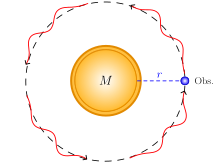
\includegraphics[width=\linewidth]{Fig-Ejercicio-1.1}
        \caption{Esquema de la situación física.}
        \label{fig:Ej-1.1}
    \end{subfigure}\hskip 1em%
    \begin{subfigure}[t]{0.48\textwidth}
        \centering
        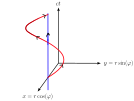
\includegraphics[width=\linewidth]{Fig-Ejercicio-1.2}
        \caption{Diagrama del espaciotiempo: línea de mundo del observador (en azul) y del fotón (en rojo).}
        \label{fig:Ej-1.2}
    \end{subfigure}
\end{figure}


\textbf{(c)} Determine las coordenadas del evento en el que la línea de mundo del rayo de luz vuelve a cruzarse con la línea de mundo del observador, luego de una revolución.

\textbf{Solución:} Después de una revolución, la línea de mundo del rayo del luz vuelve a cruzarse con la línea de mundo del observador cuando $\varphi_{\text{fot}} = 2\pi$. Por tanto, las coordenadas de este evento son
\begin{shaded}
\begin{equation}
x^{\mu} = \left(\frac{2\pi r}{\sqrt{A(r)}},r,\frac{\pi}{2},2\pi\right). \label{eq:ej-1-inter}
\end{equation}
\end{shaded}

\textbf{(d)} Determine el tiempo propio, $\tau_{\text{vuelo}}$, que el observador mide entre la ``salida" \ y la ``llegada" del fotón, luego de una revolución.

\textbf{Solución:} Después de una revolución las líneas de mundo del fotón y del observador se intersectan en el evento de coordenadas dadas por \eqref{eq:ej-1-inter}. Por lo tanto, para que coincidan \eqref{eq:ej-1-a)} y \eqref{eq:ej-1-b)}, tiene que cumplirse 
\begin{equation}
\frac{2\pi r}{\sqrt{A(r)}} = \frac{c\tau_{\text{vuelo}}}{\sqrt{A(r)}}.
\end{equation}

Despejando $\tau_{\text{vuelo}}$, encontramos que 
\begin{shaded}
\begin{equation}
\tau_{\text{vuelo}} = \frac{2\pi r}{c}. \label{eq:ej-1-d)}
\end{equation}
\end{shaded}

Notemos que el resultado es independiente de la métrica \eqref{eq:ej-1-metric}.

\textbf{(e)} El tiempo (propio) determinado en el punto anterior es una cantidad directamente medible: el ``tiempo de vuelo del fotón moviéndose en movimiento circular medido por un observador estático". A partir de este valor, llame $d := c \tau_{\text{vuelo}}$ ``distancia recorrida por el fotón moviéndose en movimiento circular, con respecto a un observador estático"\ o, alternativamente, ``perímetro de la circunferencia, con respecto a un observador estático", y determine su valor, en términos de $A$, $B$ y $r$.

\textbf{Solución:} Si definimos la ``distancia recorrida" por el fotón como $d := c \tau_{\text{vuelo}}$, obtenemos que
\begin{shaded}
\begin{equation}
d = 2\pi r, \label{eq:ej-1-e)}
\end{equation}
\end{shaded}
lo cual coincide con nuestro entendimiento clásico de perímetro de circunferencia.

\textbf{(f)} Considere, como caso particular, el espaciotiempo de Schwarzschild. Rehaga los cálculos anteriores, pero ahora en \textit{coordenadas isotrópicas}. Compare los resultados obtenidos para $d$. Comente.

\textbf{Solución:} Si consideremos el espaciotiempo de Schwarzschild:
\begin{equation}
A(r) = 1 - \frac{2m}{r}, \quad B(r) = \frac{1}{1 - \frac{2m}{r}}.
\end{equation}

La líneas de mundo del observador y del fotón se encuentran parametrizadas, respectivamente, por
\begin{align}
x_{\text{obs}}^{\mu}(\tau_\text{obs}) &= \left(\frac{c\tau_\text{obs}}{\sqrt{1 - \frac{2m}{r}}},r,\frac{\pi}{2},0 \right), \\
x_{\text{fot}}^{\mu}(\varphi_{\text{fot}}) &= \left(\frac{r}{\sqrt{1 - \frac{2m}{r}}} \varphi_{\text{fot}},r,\frac{\pi}{2},\varphi_{\text{fot}} \right).
\end{align}

El tiempo de vuelo y la distancia recorrida tienen los mismo valores \eqref{eq:ej-1-d)} y \eqref{eq:ej-1-e)}, respectivamente, porque el resultado es independiente de los coeficientes métricos $A(r)$ y $B(r)$.

Por otro lado, el elemento de línea, en \textit{coordenadas isotrópicas} $x^{\mu} = (ct,\rho,\theta,\varphi)$, está dado por
\begin{equation}
ds^2 = \frac{\left(1 - \frac{m}{2\rho} \right)^2}{\left(1 + \frac{m}{2\rho} \right)^2} c^2 dt^2 - \left( 1 + \frac{m}{2\rho}\right)^4 [d\rho^2 + \rho^2 (d\theta^2 + \sin^2\theta d\varphi^2)], \quad \rho > \frac{m}{2}. \label{eq:isotropic-metric}
\end{equation}

Las coordenadas del observador son $x_{\text{obs}}^{\mu}(\tau_{\text{obs}}) = (c t_{\text{obs}}(\tau_{\text{obs}}),\rho,\pi/2,0)$, con $\rho = \text{cte}$. Para encontrar $t_{\text{obs}}(\tau_{\text{obs}})$ debemos recordar la siguiente relación entre el tiempo propio y el elemento de línea:
\begin{equation}
c^2 d\tau^2 = ds^2 = g_{\mu\nu} dx^{\mu} dx^{\nu}.
\end{equation}

Evaluando los coeficientes de la métrica \eqref{eq:isotropic-metric} y considerando que la única coordenada no constante es $t$, tenemos que
\begin{equation}
c^2d\tau^2 = g_{tt} c^2dt^2 = \frac{\left(1 - \frac{m}{2\rho} \right)^2}{\left(1 + \frac{m}{2\rho} \right)^2} c^2 dt^2.
\end{equation} 

Despejando $dt/d\tau$:
\begin{equation}
\frac{dt}{d\tau} = \frac{\left(1 + \frac{m}{2\rho}\right)}{\left(1 - \frac{m}{2\rho}\right)} .
\end{equation}

Integrando con respecto a $\tau$:
\begin{equation}
t = \frac{\left(1 + \frac{m}{2\rho}\right)}{\left(1 - \frac{m}{2\rho}\right)} \tau + C,
\end{equation}
donde $C$ es una constante de integración. Si asumimos que el observador se encuentra en el evento $x^{\mu} = (0,\rho,\pi/2,0)$ para $\tau = 0$, se fija la constante $C$ a cero. Entonces, renombrando las variables $t \to t_{\text{obs}}$ y $\tau \to \tau_{\text{obs}}$, 
\begin{equation}
t_{\text{obs}}(\tau_\text{obs}) = \frac{\left(1 + \frac{m}{2\rho}\right)}{\left(1 - \frac{m}{2\rho}\right)} \tau_\text{obs}.
\end{equation}

Por lo tanto, la línea de mundo del observador se encuentra parametrizada por
\begin{shaded}
\begin{equation}
x_{\text{obs}}^{\mu}(\tau_\text{obs}) = \left(\frac{\left(1 + \frac{m}{2\rho}\right)}{\left(1 - \frac{m}{2\rho}\right)} c \tau_{\text{obs}},\rho,\frac{\pi}{2},0 \right). \label{eq:ej-1-f.1)}
\end{equation}
\end{shaded}

Las coordenadas del fotón son $x_{\text{fot}}^{\mu}(\lambda) = (ct_{\text{fot}}(\lambda),\rho,\pi/2,\varphi_{\text{fot}}(\lambda))$. Elegimos parametrizar su línea de mundo por $\lambda = \varphi_{\text{fot}}$. 

Usando la condición de curvas nulas para el fotón:
\begin{equation}
ds^2|_{\text{fot}} = g_{\mu\nu} dx^{\mu}dx^{\nu} = 0.
\end{equation}

Evaluamos los coeficientes de la métrica \eqref{eq:isotropic-metric}  considerando que las únicas coordenadas no constantes son $ct$ y $\varphi$,
\begin{align}
g_{\mu\nu} dx^{\mu}dx^{\nu} &= 0 \\
g_{tt} c^2dt^2 + g_{\rho\rho} \CancelTo[\color{red}]{0}{d\rho^2} + g_{\theta\theta} \CancelTo[\color{red}]{0}{d\theta^2} + g_{\varphi\varphi} d\varphi^2 &= 0 \\
\frac{\left(1 - \frac{m}{2\rho} \right)^2}{\left(1 + \frac{m}{2\rho} \right)^2} c^2 dt^2 - \left(1 + \frac{m}{2\rho} \right)^4 \rho^2 \sin^2\left( \frac{\pi}{2} \right)d\varphi^2 &= 0 \\
c^2dt^2 &= \frac{\left(1 + \frac{m}{2\rho}\right)^6}{\left(1 - \frac{m}{2\rho}\right)^2} \rho^2 \,d\varphi^2 \\
c \frac{dt}{d\varphi}&=  \frac{\left(1 + \frac{m}{2\rho}\right)^3}{\left(1 - \frac{m}{2\rho}\right)} \rho.
\end{align}

Integrando con respecto a $\varphi$:
\begin{align}
\int c \frac{dt}{d\varphi} d\varphi &= \int \frac{\left(1 + \frac{m}{2\rho}\right)^3}{\left(1 - \frac{m}{2\rho}\right)} \rho d\varphi \\
ct &= \frac{\left(1 + \frac{m}{2\rho}\right)^3}{\left(1 - \frac{m}{2\rho}\right)} \rho \varphi + D,
\end{align}
donde $D$ es una constante de integración. Si asumimos que el fotón pasa por el evento con coordenadas $x^{\mu}(0) = (0,\rho,\pi/2,0)$, se fija la constante $D$ a cero. Entonces, renombrando las variables $t \to t_{\text{fot}}$ y $\varphi\to\varphi_{\text{fot}}$, hemos encontrado que
\begin{equation}
ct_{\text{fot}} = \frac{\left(1 + \frac{m}{2\rho}\right)^3}{\left(1 - \frac{m}{2\rho}\right)} \rho \varphi_{\text{fot}}.
\end{equation}

Por lo tanto, la línea de mundo se encuentra parametrizada por
\begin{shaded}
\begin{equation}
x_{\text{fot}}^{\mu}(\varphi_{\text{fot}}) = \left(\frac{\left(1 + \frac{m}{2\rho}\right)^3}{\left(1 - \frac{m}{2\rho}\right)} \rho \varphi_{\text{fot}},\rho,\frac{\pi}{2},\varphi_{\text{fot}} \right). \label{eq:ej-1-f.2)}
\end{equation}
\end{shaded}

Después de una revolución, la línea de mundo del rayo del luz vuelve a cruzarse con la línea de mundo del observador cuando $\varphi_{\text{fot}} = 2\pi$. Por tanto, las coordenadas de este evento son
\begin{equation}
x^{\mu} = \left(\frac{\left(1 + \frac{m}{2\rho}\right)^3}{\left(1 - \frac{m}{2\rho}\right)} 2\pi \rho,\rho,\frac{\pi}{2},2\pi\right). \label{eq:ej-1-f.3)}
\end{equation}

Por lo tanto, para que coincidan \eqref{eq:ej-1-f.1)} y \eqref{eq:ej-1-f.2)}, se debe cumplir que
\begin{equation}
\frac{\left(1 + \frac{m}{2\rho}\right)^3}{\left(1 - \frac{m}{2\rho}\right)} 2\pi \rho = \frac{\left(1 + \frac{m}{2\rho}\right)}{\left(1 - \frac{m}{2\rho}\right)} c \tau_{\text{vuelo}}
\end{equation}  

Despejando $\tau_{\text{vuelo}}$, encontramos que 
\begin{shaded}
\begin{equation}
\tau_{\text{vuelo}} = \frac{2\pi \rho}{c} \left(1 + \frac{m}{2\rho}\right)^2. \label{eq:ej-1-f.4)}
\end{equation}
\end{shaded}

Luego, la ``distancia recorrida" por el fotón \ es
\begin{shaded}
\begin{equation}
d = c \tau_{\text{vuelo}} = 2\pi \rho \left(1 + \frac{m}{2\rho}\right)^2, \label{eq:ej-1-f.5)}
\end{equation}
\end{shaded}
la cual es distinta que la ``distancia" en coordenadas de curvatura.

Como el tiempo propio es un escalar, podemos igualar las ecuaciones \eqref{eq:ej-1-d)} y \eqref{eq:ej-1-f.4)}, obteniendo 
\begin{equation}
r = \rho \left(1 + \frac{m}{2\rho}\right)^2,
\end{equation}
la cual corresponde a la transformación entre las coordenadas $r$ y $\rho$ vistas en el documento de la semana 1.

\section*{Ejercicio 2:}

Considere un objeto orbitando una masa esféricamente simétrica, en una órbita geodésica circular ($r = R = \text{cte}$), un observador comóvil y dos observadores ``en reposo", todos ubicados en el mismo plano de la órbita, tal como se describen más abajo. Modele el problema usando la métrica de Schwarzschild en coordenadas de curvatura:
\begin{equation}
ds^2 = \left( 1 - \frac{2m}{r}\right) c^2dt^2 - \frac{dr^2}{\left( 1 - \frac{2m}{r} \right)} - r^2 [d\theta^2 + \sin^2\theta d\varphi^2], \quad r > 2m. \label{eq:Schwarzschild-metric}
\end{equation}


\textbf{(a)} Determine el tiempo $T_{\text{com}}$, que mide un observador viajando (es decir, comóvil) con el cuerpo que orbita, en una revolución, en función de la coordenada radial $R$ de la órbita.
\\

\textbf{Solución:} Sabemos del documento de la semana 3 que una geodésica circular estable con coordenada radial $r_{\text{c}}$, parametrizada por el tiempo propio, está dada por
\begin{equation}
x^{\mu}(\tau) = \left(\frac{c\tau}{\sqrt{1 - \frac{3m}{r_{\text{c}}}}}, r_{\text{c}}, \frac{\pi}{2}, \frac{c\tau}{r_{\text{c}}} \sqrt{\frac{m}{r_{\text{c}} - 3m}} \right). \label{eq:coord-obs1}
\end{equation}

En nuestro caso, $r_{\text{c}} = R$. El tiempo $\tau = T_{\text{com}}$ que mide un observador viajando con el cuerpo que orbita, en una revolución, se obtiene cuando la coordenada angular $\varphi = 2\pi$, ésto es,
\begin{equation}
\frac{cT_{\text{com}}}{R} \sqrt{\frac{m}{R - 3m}} = 2\pi.
\end{equation}

Despejando $T_{\text{com}}$, encontramos que
\begin{shaded}
\begin{equation}
T_{\text{com}} =  \frac{2\pi R}{c} \sqrt{\frac{R-3m}{m}}.  \label{eq:ej-2-a)}
\end{equation}
\end{shaded}

Si consideremos el límite de campo débil: $R \gg m$, 
\begin{equation}
T_{\text{com}} \approx  \frac{2\pi R}{c} \sqrt{\frac{R}{m}} = 2\pi \sqrt{\frac{R^3}{GM}}, 
\end{equation}
donde se reemplazó $m = GM/c^2$. Este resultado coincide con el caso newtoniano. En efecto, para un cuerpo de masa $\bar{m}$ que describe un movimiento circular de radio $R$ producto de la fuerza de atracción gravitatoria, por la segunda ley de Newton,
\begin{equation}
\frac{GM\bar{m}}{R^2} = \bar{m} a_{\text{cen}} = \bar{m} R \omega^2,
\end{equation}
con $a_{\text{cen}} = R\omega^2$ la aceleración centrípeta. Recordando que $\omega = 2\pi/T$, tenemos que
\begin{equation}
\omega^2 = \frac{GM}{R^3} \Rightarrow T = 2\pi \sqrt{\frac{R^3}{GM}}. \label{eq:period-newton}
\end{equation}

\textbf{(b)} Determine ahora el tiempo $T_{\text{rep}}$, que mide un observador ``en reposo"\ e igualmente distanciado del centro de fuerzas que el objeto orbitando (es decir, con la misma coordenada radial) en una revolución.
\\

\textbf{Solución:} Las coordenadas del observador ``en reposo" son $x_{\text{rep}}^{\mu} = (ct,R,\pi/2,0)$. Usando la relación entre el tiempo propio y el elemento de línea:
\begin{equation}
c^2d\tau^2 = ds^2 = g_{\mu\nu} dx^{\mu}dx^{\nu}.
\end{equation}

Evaluando los coeficientes de la métrica \eqref{eq:Schwarzschild-metric} y considerando que la única coordenada no constante es $t$, tenemos que 
\begin{equation}
c^2d\tau^2 = g_{tt} c^2 dt^2 = \left( 1 - \frac{2m}{R}\right) c^2dt^2.
\end{equation}

Despejando $dt/d\tau$:
\begin{equation}
\frac{dt}{d\tau} = \frac{1}{\sqrt{1 - \frac{2m}{R}}}.
\end{equation}

Integrando con respecto a $\tau$:
\begin{equation}
t = \frac{\tau}{\sqrt{1 - \frac{2m}{R}}} + D,
\end{equation}
donde $D$ es una constante de integración. Si asumimos que el observador en reposo para por el evento de coordenadas $x^{\mu} = (0,R,\pi/2,0)$ para $\tau = 0$, se fija la constante $D$ a cero. Por tanto, renombrando las variables $t \to t_{\text{rep}}$ y $\tau \to \tau_{\text{rep}}$,
\begin{equation}
t_{\text{rep}} = \frac{\tau_{\text{rep}}}{\sqrt{1 - \frac{2m}{R}}}.
\end{equation}

Por lo tanto, la línea de mundo del observador en reposo se encuentra parametrizada por
\begin{equation}
x_{\text{rep}}^{\mu}(\tau_{\text{rep}}) = \left(\frac{c\tau_{\text{rep}}}{\sqrt{1 - \frac{2m}{R}}},R,\frac{\pi}{2},0 \right). \label{eq:coord-obs2}
\end{equation}

Después de una revolución, las líneas de mundo del observador orbitando y en reposo se intersectan, coincidiendo sus coordenadas temporales. Reemplazando $\tau$ por $T_{\text{com}}$ en \eqref{eq:coord-obs1}, tenemos que 
\begin{align}
\frac{cT_{\text{com}}}{\sqrt{1 - \frac{3m}{R}}} &= \frac{c}{\sqrt{1 - \frac{3m}{R}}} \frac{2\pi R}{c} \sqrt{\frac{R-3m}{m}} \nonumber\\
&= \frac{2\pi R}{\sqrt{\frac{R-3m}{R}}} \sqrt{\frac{R-3m}{m}} \nonumber\ \\
&= 2\pi \sqrt{\frac{R^3}{m}}.
\end{align}

Entonces, igualando la coordenada temporal del observador orbitando y del observador en reposo:
\begin{align}
\frac{cT_{\text{com}}}{\sqrt{1 - \frac{3m}{R}}} &= \frac{cT_{\text{rep}}}{\sqrt{1 - \frac{2m}{R}}} \\
2\pi \sqrt{\frac{R^3}{m}} &= \frac{cT_{\text{rep}}}{\sqrt{1 - \frac{2m}{R}}}  \\
T_{\text{rep}} &= \frac{2\pi}{c} \sqrt{1 - \frac{2m}{R}} \sqrt{\frac{R^3}{m}} \\
T_{\text{rep}} &= \frac{2\pi}{c} \sqrt{\frac{R^3}{m} - 2R^2}.
\end{align}

Reordenando la última expresión, tenemos que el tiempo que mide un observador en reposo es 
\begin{shaded}
\begin{equation}
T_{\text{rep}} = \frac{2\pi R}{c} \sqrt{\frac{R-2m}{m}}. \label{eq:ej-2-b)}
\end{equation}
\end{shaded}

\textbf{(c)} Finalmente, determine el tiempo $T_{\infty}$ que mide un observador ``en reposo" muy lejano (``en el infinito"), es decir, con $r = \text{cte}$, pero $r \gg 2m$, correspondiente a cuando él ``ve" que el objeto orbitando finaliza una revolución completa.
\\

\textbf{Solución:} Si consideremos que los observadores están alineados, podemos usar la expresión calculada para el redshift gravitacional en el documento de la semana 6, a saber,
\begin{equation}
\frac{\Delta \tau_\text{r}}{\Delta \tau_{\text{e}}} = \sqrt{\frac{1 - \frac{2m}{r_{\text{R}}}}{1 - \frac{2m}{r_{\text{E}}}}}.
\end{equation}

En nuestro caso, $r_{\text{R}} \gg 2m$, $r_{\text{E}} = R$, $\Delta \tau_\text{r} = T_{\infty}$ y $\Delta \tau_\text{e} = T_{\text{rep}}$. Por tanto,
\begin{equation}
\frac{T_{\infty}}{T_{\text{rep}}} = \frac{1}{\sqrt{1 - \frac{2m}{R}}}. \label{eq:ej-2-c.1)}
\end{equation}

Reemplazando \eqref{eq:ej-2-b)} en \eqref{eq:ej-2-c.1)}, tenemos que
\begin{align}
T_{\infty} &= \frac{T_{\text{rep}}}{\sqrt{1 - \frac{2m}{R}}} \nonumber \\
&= \frac{1}{\sqrt{1 - \frac{2m}{R}}} \left( \frac{2\pi R}{c} \sqrt{\frac{R-2m}{m}} \right) \nonumber \\
&= \frac{2\pi R}{c}\frac{\sqrt{R}}{\sqrt{R-2m}} \frac{\sqrt{R-2m}}{\sqrt{m}} \nonumber \\
&= \frac{2\pi}{c} \sqrt{\frac{R^3}{m}}.
\end{align}

Por lo tanto, el tiempo que mide un observador en reposo en el infinito es 
\begin{shaded}
\begin{equation}
T_{\infty} = \frac{2\pi}{c} \sqrt{\frac{R^3}{m}}.
\end{equation}
\end{shaded}

\textbf{(d)} Los tres tiempo calculados anteriores corresponden a la noción clásica de ``periodo orbital". Compare sus resultados y discuta sus diferencias.
\\

\textbf{Solución:} Los tiempos calculados son:
\begin{align}
T_{\text{com}} &= \frac{2\pi R}{c} \sqrt{\frac{R-3m}{m}}, \\
T_{\text{rep}} &= \frac{2\pi R}{c} \sqrt{\frac{R-2m}{m}}, \\
T_{\infty} &= \frac{2\pi}{c} \sqrt{\frac{R^3}{m}}.
\end{align}

A pesar de haber sido calculados con la misma noción clásica de ``periodo orbital", sus valores son distintos. Solo el último coincide con el periodo orbital newtoniano \eqref{eq:period-newton}.

\end{document}
